% IF YOU ARE USING OVERLEAF, MAKE SURE TO SET THE COMPILER TO XeLatex (Menu in the top left > Settings > Compiler).

% Gemini theme
% See: https://rev.cs.uchicago.edu/k4rtik/gemini-uccs
% A fork of https://github.com/anishathalye/gemini

\documentclass[final]{beamer}

% ====================
% Packages
% ====================

\usepackage[T1]{fontenc}
\usepackage{lmodern}
\usepackage[size=custom,width=120,height=72,scale=1.0]{beamerposter}
\usetheme{gemini}
\usecolortheme{stanford}
\usepackage{graphicx}
\usepackage{booktabs}
\usepackage{tikz}
\usepackage{listings}
\usepackage{xcolor}
\usepackage{multicol}
\usetikzlibrary{arrows.meta,positioning,shapes.geometric,fit,backgrounds,calc}

% Compact lists without enumitem (conflicts with beamer)
\setlength{\leftmargini}{1.2em}
\setlength{\leftmarginii}{1em}
\setlength{\itemsep}{0.3ex}
\setlength{\parsep}{0pt}

\lstset{
  basicstyle=\ttfamily\scriptsize,
  backgroundcolor=\color{gray!8},
  frame=single,
  framerule=0.4pt,
  rulecolor=\color{gray!40},
  breaklines=true,
  columns=fullflexible,
  keepspaces=true,
  aboveskip=4pt,
  belowskip=4pt,
}

% ====================
% Lengths
% ====================

\newlength{\sepwidth}
\newlength{\colwidth}
\setlength{\sepwidth}{0.025\paperwidth}
\setlength{\colwidth}{0.3\paperwidth}


\title{Recursive Self-Improvement for Continual Adaptation in Code Generation}

\author{
  Aaditya Nalawade \inst{1} \and Ethan Goodhart \inst{1} \and Chandra Suda \inst{1} \\[0.3em]
  \textbf{Mentor:} Minsik Oh
}

\institute[shortinst]{\inst{1} Department of Computer Science, Stanford University}

\footercontent{
  \href{mailto:aaditya1@stanford.edu}{aaditya1@stanford.edu} \textbullet{}
  \href{mailto:goodhart@stanford.edu}{goodhart@stanford.edu} \textbullet{}
  \href{mailto:csuda@stanford.edu}{csuda@stanford.edu} \hfill
  CS224N Custom Project, Winter 2026 \hfill
  }

\begin{document}

\addtobeamertemplate{headline}{}
{
    \begin{tikzpicture}[remember picture,overlay]
      \node [anchor=north east, inner sep=3cm] at ([xshift=0.0cm,yshift=2.5cm]current page.north east)
      {
\includegraphics[height=7.0cm]{stanford_logos/Block_S_2_color.png}};
    \end{tikzpicture}
}

\begin{frame}[t]
\begin{columns}[t]
\begin{column}{\sepwidth}\end{column}

% ====================
% COLUMN 1: Motivation + Architecture
% ====================
\begin{column}{\colwidth}

\begin{block}{Motivation}

\textbf{Problem:} Deployed LLMs need continual learning without forgetting, but Self-Distilled Policy Optimization (SDPO) requires golden solutions and updates indiscriminately.

\textbf{Our idea:} \textbf{Recursive self-improvement} --- bootstrap improvement using \emph{only} a test-case verifier (no golden solutions ever provided). The model:
\begin{itemize}[]
  \item Generates solutions, recursively refines failures
  \item Distills self-discovered successes into its own weights
  \item Externalizes lessons into a retrievable memory (RAG)
  \item Routes its own learning via prompt-based tool calls
\end{itemize}

\textbf{Key question:} Can a model teach itself from verifier feedback alone?

\end{block}

\begin{block}{System Architecture}

\begin{figure}[h]
\centering
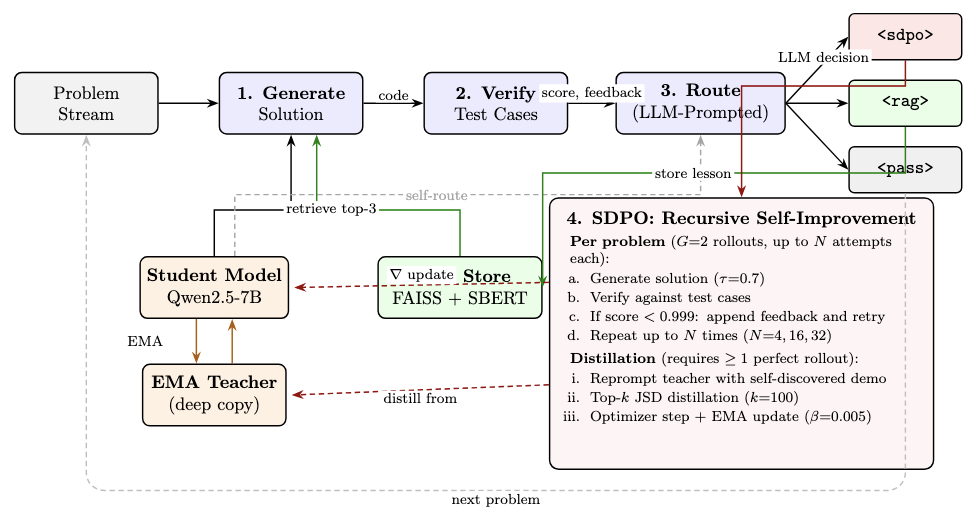
\includegraphics[width=0.98\textwidth]{diagram.png}
\end{figure}

\vspace{-1ex}
\textbf{Components:} \textbf{Student} (Qwen2.5-7B-Instruct), \textbf{EMA Teacher} (deep copy, $\beta{=}0.005$), \textbf{RAG} (FAISS + SBERT), \textbf{Router} (LLM-prompted self-route)

\end{block}

\begin{block}{Recursive Self-Improvement Loop}

\textbf{Phase 1: Rollout generation} --- For each problem, $G{=}2$ independent rollouts. Each rollout:
\begin{enumerate}[]
  \item Generate solution ($\tau{=}0.7$)
  \item Verify against test suite
  \item If $<99.9\%$: append structured feedback to cumulative \emph{feedback window}
  \item Re-prompt: ``Analyze errors above, choose DIFFERENT algorithm, do NOT repeat failed logic''
  \item Repeat up to $N$ times ($N \in \{4,16,32\}$)
\end{enumerate}

\textbf{Phase 2: Distillation} --- Only rollouts $\geq99.9\%$ proceed. Teacher reprompted with: (a) original problem, (b) self-discovered correct solution, (c) initial failure feedback. Top-$k$ JSD distillation ($k{=}100$, $\alpha{=}0.5$). No reference KL ($\beta_{\text{ref}}{=}0$) $\Rightarrow$ saves $\sim$14GB VRAM.

\textbf{Phase 3: Optimizer} --- 8-bit AdamW, $lr{=}2{\times}10^{-6}$, grad clip 1.0. EMA: $\theta_t \leftarrow (1{-}\beta)\theta_t + \beta\theta_s$, $\beta{=}0.005$.

\textbf{Teacher's advantage:} Sees correct solution discovered via recursion --- distills ``shortcut'' knowledge back to student.

\end{block}

\end{column}
\begin{column}{\sepwidth}\end{column}

% ====================
% COLUMN 2: RAG + Results Tables
% ====================
\begin{column}{\colwidth}

\begin{block}{RAG Knowledge Store}

When router selects \texttt{<rag>}: model generates concise lesson (2--3 sentences, \emph{type} of mistake not specific code) + truncated problem summary. Stored in FAISS \texttt{IndexFlatIP} with Sentence-BERT (\texttt{all-MiniLM-L6-v2}). During generation: top-3 by cosine similarity prepended as system context.

\textbf{Example stored chunk:}

{\scriptsize\texttt{Problem summary: Given string s of lowercase letters...}}\\
{\scriptsize\texttt{Lesson: The solution processed the entire string in one pass without managing time complexity, causing TLE. In similar problems, avoid nested substring ops that scale poorly with input size.}}

\textbf{Why RAG underperforms in our regime:} Only $\sim$20--30 chunks by step 200. Sparse coverage $\Rightarrow$ retrieval adds noise, not signal. This is a \emph{scale limitation}, not conceptual failure. SDPO-only $>$ SDPO+RAG currently.

\end{block}

\begin{block}{Main Results (50 test problems, best checkpoint)}

\begin{table}
\centering
\small
\begin{tabular}{lccc}
\toprule
\textbf{Configuration} & \textbf{Test-Case Acc} & \textbf{Solve Rate} & \textbf{Correct}\\
\midrule
Baseline (Qwen 7B) & 51.3\% & 32\% & 16/50\\
\midrule
\multicolumn{4}{l}{\textit{7B, v1 ($N{=}4$)}}\\
\quad SDPO-only & \textbf{55.9\%} & \textbf{38\%} & \textbf{19/50}\\
\quad RAG+SDPO & 52.0\% & 34\% & 17/50\\
\midrule
\multicolumn{4}{l}{\textit{7B, v2 ($N{=}16$)}}\\
\quad SDPO-only & 55.5\% & 30\% & 15/50\\
\quad RAG+SDPO & 47.6\% & 32\% & 16/50\\
\midrule
\multicolumn{4}{l}{\textit{7B, v3 ($N{=}32$)}}\\
\quad SDPO-only & 53.0\% & 30\% & 15/50\\
\quad RAG+SDPO & 47.2\% & 28\% & 14/50\\
\midrule
Baseline (Qwen 1.5B) & 14.0\% & 14\% & 7/50\\
\quad 1.5B + SDPO & 8.0\% & 8\% & 4/50\\
\quad 1.5B + RAG+SDPO & 10.0\% & 10\% & 5/50\\
\bottomrule
\end{tabular}
\caption*{\scriptsize \textbf{Key:} +6\,pp solve rate from pure self-improvement. 1.5B \emph{degrades} $\Rightarrow$ minimum capability threshold.}
\end{table}

\textbf{v1 checkpoint progression:}
\begin{table}
\centering
\small
\begin{tabular}{ccccc}
\toprule
\textbf{Step} & \textbf{SDPO Acc} & \textbf{SDPO Solve} & \textbf{RAG+SDPO Acc} & \textbf{RAG+SDPO Solve}\\
\midrule
50 & 54.4\% & 32\% & 50.8\% & 32\%\\
100 & \textbf{56.5\%} & 36\% & 53.6\% & 34\%\\
150 & 54.9\% & 36\% & \textbf{53.9\%} & 34\%\\
200 & 55.9\% & \textbf{38\%} & 51.8\% & 34\%\\
250 & 52.9\% & 36\% & 54.9\% & 32\%\\
\bottomrule
\end{tabular}
\caption*{\scriptsize Baseline: 51.3\% acc, 32\% solve. Peak at step 200.}
\end{table}

\end{block}

\begin{block}{The Attempt-Count Paradox}

\textbf{Finding:} More recursive attempts $\Rightarrow$ more training-time perfect rollouts, but \textbf{worse} evaluation generalization.

\begin{table}
\centering
\small
\begin{tabular}{lccccc}
\toprule
\textbf{Config} & \textbf{Perfects} & \textbf{Att. 1} & \textbf{Att. $>$1} & \textbf{\% from $>$1} & \textbf{Eval Solve}\\
\midrule
v1 ($N{=}4$) & 106 & 40 & 66 & 62\% & \textbf{38\%}\\
v2 ($N{=}16$) & 54 & 11 & 43 & 80\% & 30\%\\
v3 ($N{=}32$) & 67 & 11 & 56 & 84\% & 30\%\\
\bottomrule
\end{tabular}
\caption*{\scriptsize 84\% of v3 perfects from recursion, yet v3 solves \textbf{worse} than v1.}
\end{table}

\textbf{Interpretation:} Deep retry loops encourage \textbf{locally patched} solutions (hardcoding test-specific fixes) rather than algorithmic corrections. These overfit to training feedback, transfer poorly.

\end{block}

\end{column}
\begin{column}{\sepwidth}\end{column}

% ====================
% COLUMN 3: Analysis + Takeaways
% ====================
\begin{column}{\colwidth}

\begin{block}{Key Findings}

\begin{itemize}[]
  \item[\textcolor{cardinalred}{$\bullet$}] \textbf{Verifier-only self-improvement works:} +6\,pp solve rate (32\%$\to$38\%) on LiveCodeBench with \textbf{no golden solutions, no external demonstrations}.
  \item[\textcolor{cardinalred}{$\bullet$}] \textbf{Minimum capability threshold:} 1.5B model actively degrades under same pipeline. Self-distillation requires sufficient base competence.
  \item[\textcolor{cardinalred}{$\bullet$}] \textbf{SDPO $>$ RAG here:} With $\sim$20--30 stored lessons, retrieval lacks semantic density. Memory scale issue, not conceptual failure.
  \item[\textcolor{cardinalred}{$\bullet$}] \textbf{Paradox of depth:} More training-time recovery (84\% perfects from recursion at $N{=}32$) but worse eval. Recursive patching overfits.
\end{itemize}

\textbf{Routing breakdown (v1, 500 problems):}
\begin{itemize}[]
  \item 52\% $\to$ SDPO (261 problems)
  \item 14\% $\to$ RAG (69 problems)
  \item 34\% $\to$ PASS (170 problems) --- consistent with 32\% baseline
\end{itemize}

\textbf{Failure mode at high $N$:} With 16/32 attempts, model increasingly hardcodes expected outputs for specific inputs rather than fixing algorithmic logic. Recursive feedback loop amplifies this. Future: richer feedback (CoT ``why wrong'').

\end{block}

\begin{block}{Training Details}

\begin{itemize}[]
  \item \textbf{Data:} LiveCodeBench (924 problems, 70/30 split, 50-test subsample)
  \item \textbf{Hardware:} NVIDIA H100 via Modal; BFloat16; gradient checkpointing
  \item \textbf{Wall-clock:} v1 6h12m (500 probs), v2 11h11m (250 probs), v3 11h10m (200 probs)
  \item \textbf{Hyperparams:} $lr{=}2{\times}10^{-6}$, 8-bit AdamW, top-$k{=}100$, $\alpha{=}0.5$, $\beta{=}0.005$, $\beta_{\text{ref}}{=}0$, $G{=}2$, $N{\in}\{4,16,32\}$
\end{itemize}

\textbf{Contributions:}
\begin{itemize}[]
  \item Aaditya Nalawade: SDPO implementation, top-$k$ JSD loss, EMA teacher, Modal training
  \item Ethan Goodhart: Training loop, model architecture, experimental design, paper writing
  \item Chandra Suda: RAG store, prompt-based router, verification pipeline, evaluation framework
\end{itemize}

\end{block}

\begin{block}{References}

\scriptsize
\vspace{-1ex}
\begin{multicols}{2}
\nocite{*}
\bibliographystyle{unsrt}
\bibliography{poster}
\end{multicols}

\end{block}

\end{column}

\begin{column}{\sepwidth}\end{column}
\end{columns}
\end{frame}

\end{document}
